% !TeX spellcheck = ru_RU
% !TEX root=../main.tex

\begin{lecture}[Ионные пары]
	\begin{lecSection}[Типы ионных пар]
			\begin{figure}[H]
			\begin{minipage}[h]{0.26\linewidth}
				\centering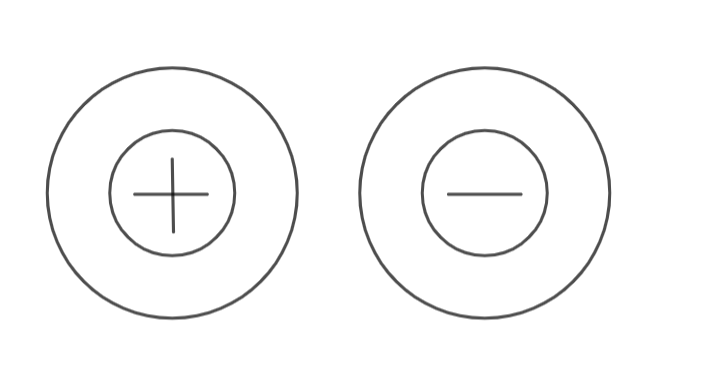
\includegraphics[width=\linewidth]{lecture_06/pic1}
				\caption{Свободная ионная пара}
			\end{minipage}
			\hfill
			\begin{minipage}[h]{0.30\linewidth}
				\centering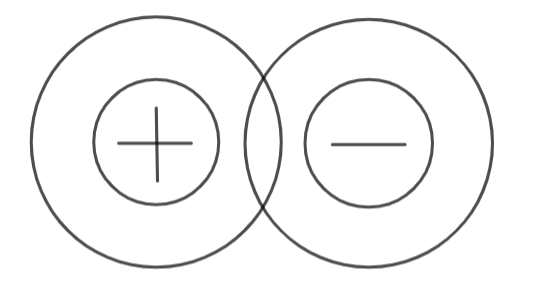
\includegraphics[width=\linewidth]{lecture_06/pic2}
				\caption{Сольватно-разделенные ионные пары(катионы и анионы образуют сольватные оболочки)}
			\end{minipage}
			\hfill
			\begin{minipage}[h]{0.28\linewidth}
				\centering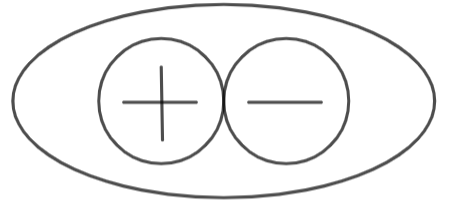
\includegraphics[width=\linewidth]{lecture_06/pic3}
				\caption{Контактная пара($r \leq 10$ \AA)}
			\end{minipage}
	\end{figure}
К-пары и С-пары по-разному участвуют в химических реакциях.
\par Проводимость, подвижность, радиус ионов оценивается с опорой на формулу Стокса.

\begin{center}
\begin{tabular}{|c|c|c|}
	\hline 
	Вещество & $\eta$, сП & $q_{статич}$ \\ 
	\hline 
	вода & 1 & 80 \\ 
	\hline 
	спирт & 1 & 20 \\ 
	\hline 
	ДМСО & 2 & 0 \\ 
	\hline 
	бензол & 0,6 & 2 \\ 
	\hline 
\end{tabular}
 \end{center}

	\end{lecSection}

	\begin{lecSection}[Механизм Айгена]
		
		$\mathrm{C^+S_m + A^-S_n \rightleftharpoons S_pC^+S_2A^-S_q \rightleftharpoons S_rC^+SA^-S_1 \rightleftharpoons S_x(C^+A^-)S_y}$, где $\mathrm{C^+}$ - катион, $\mathrm{A^+}$ - анион, $\mathrm{S}$ - сольвент, $m, n, p, r, x, y$ - числа сольватаци.
		\par Для дипольного масштаба: $l \sim 1$ \AA, $m = 4,8 D \rightarrow 4,8$ Дебай $= 4,8 \cdot 10^{-10} \cdot 10^{-8} \simeq 4,8 \cdot 10^{-18}$ СГС(1 Дебай = $10^{-18}$ СГС).
		\begin{center}
			\begin{tabular}{|c|c|}
				\hline 
				Вещество & $m, D$ \\ 
				\hline 
				вода & 1,8 \\ 
				\hline 
				бензол & 0 \\ 
				\hline 
				ДМСО & 4 \\ 
				\hline 
			\end{tabular} 
		\end{center}
	У ДМСО сильное взаимодействие между молекулами.
		
	\end{lecSection}

	\begin{lecSection}[Виды взаимодействия между частицами]
		
		\subsection{1. Взаимодействие ион-ион}
		
		$\dfrac{Z_AZ_Be^2}{\varepsilon r} \sim kT, R_0 = \dfrac{e^2}{\varepsilon kT}$ - радиус Онзагера.
		\par Пример:
		\par $kT \simeq \dfrac{1}{40}$ эВ, $Rg = \dfrac{e^2}{2 a_0} \simeq 13,6$ эВ $ \rightarrow \dfrac{R_0}{2a_0} = \dfrac{e^2}{\varepsilon 2a_0 kT} = \dfrac{Rg}{\varepsilon kT} \simeq 55$ \AA.

		\subsection{2. Взаимодействие ион-диполь}
		
		$l = -mE_x = - \dfrac{Zem}{\varepsilon R^2}$
		
		\subsection{3. Взаимодействие ион-нейтральная частица}
		
		$E_x = \dfrac{Zl}{\varepsilon R^2} \rightarrow m = \alpha l \rightarrow l = -m E_x = - \alpha \dfrac{Z^2e^2}{\varepsilon^2 R^4}$, уже короткодействующая сила.
		
		\subsection{4. Взаимодействие между нейтральными частицами - Ван-дер-Ваальса}
		
		$E_x \sim \dfrac{m_B}{\epsilon R^3} \rightarrow l \sim \dfrac{m_Am_B}{\varepsilon R^3}$, $<m_B> = 0, <m_B^2> \neq 0$
		\par $m_A = \sum\limits_{\omega} m_{\omega} e^{i\omega t} \rightarrow l_{\omega} = \dfrac{m \omega}{R^3} \rightarrow l = -\sum\limits_{\omega}m\omega l_{\omega} = -\sum\limits_{\omega} \alpha \omega l_{\omega}^2 \sim \dfrac{1}{R^6}$
		\par Отсюда и получается потенциал Леонарда-Джонса.
				
	\end{lecSection}		
\end{lecture}